\section{Method}
\subsection{The Metropolis algorithm}
In order to make the models evolve in time, which is necessary to observe their dynamics, we use the well-known metropolis algorithm \cite{Metropolis1953}. For models with a defined Hamiltonian, the Metropolis algorithm proceeds as follows:
\begin{enumerate}
    \item Start from an initial configuration $\{S_i\}$.
    \item Repeat $N$ times:
    \begin{enumerate}[label=\alph*.]
        \item Pick a random spin $S_k$ and compute the energy change $\Delta E_k$
              upon flipping it.
        \item If $\Delta E_k \leq 0$, accept the flip.
        \item Else, draw a random number $r \sim \mathcal{U}([0,1])$
              and accept the flip if $r \leq e^{-\beta \Delta E_k}$.
    \end{enumerate}
    \item Repeat Step 2 for $N_{\text{sweeps}}$ sweeps.
\end{enumerate}
Where $N$ is the number of spins, $\beta$ is the inverse temperature,
and $N_{\text{sweeps}}$ is the number of sweeps, where one sweep consists of
$N$ successive single-spin flip attempts.\\
This algorithm however becomes computationally demanding when one attempts to sample a large number of configurations. This situation occurs, for example, when looking for rare samples in the dynamics, or sampling many different initial conditions -- both of which we will try to explore during this internship. We thus need to find way of optimizing the implementation of the algorithm.
\subsection{First optimization: the bitwise arithmetic}
The first optimization in the implementation of the Metropolis algorithm is the use of bitwise arithmetic. The main idea is to leverage the boolean representation as stored in our computers. The typical object that we manipulate is called \Bits: it is a collection of $n_\text{bits}=64$ boolean variables. In that way, we have the possibility to simulate $64$ evolutions of the same variable in parallel.
\nolinenumbers
\begin{figure}[ht]
\centering
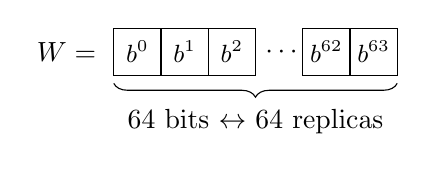
\begin{tikzpicture}

\def\boxw{0.6} % largeur exacte de la boîte
\def\step{\boxw} % PAS = largeur => boîtes collées

% left boxes
\foreach \i/\label in {0/0, 1/1, 2/2} {
    \draw (\i*\step, 0) rectangle (\i*\step+\boxw, 0.6);
    \node[font=\small] at (\i*\step+0.3, 0.3) {$b^{\label}$};
}
% ...
\node at (3*\step+0.33, 0.3) {$\cdots$};

% right boxes
\foreach \i/\label in {0/62, 1/63} {
    \draw (4*\step + \i*\step, 0)
        rectangle (4*\step + \i*\step+\boxw, 0.6);
    \node[font=\small] at (4*\step + \i*\step+0.3, 0.3)
        {$b^{\label}$};
}

% left label
\node at (-0.6, 0.3) {$W=$};

% Brace below
\draw[decorate, decoration={brace, amplitude=5pt, mirror}]
    (0, -0.1) --
    (6*\step, -0.1)
    node[midway, below=6pt] {64 bits $\leftrightarrow$ 64 replicas};

\end{tikzpicture}
\caption{A \Bits $W$ encoding 64 parallel replicas. Each bit $b^k$ carries the state of replica $k$.}
\label{fig:Bits}
\end{figure}
\linenumbers
This structure is very convenient to represent binary variable such as the spins of the system. The boolean representation $b^k \in \{0,1\}$ of a spin $s^k \in \{-1,+1\}$ is given by $b^k = (s^k+1)/2$. In that way, we are able to implement several replicas of the full spin system in a set of \Bits $\{S_i\}$, each encoding the replicas of the associated spin, as shown in Figure~\ref{fig:spins_Bits}.
\nolinenumbers
\begin{figure}[t]
\centering
\def\svgwidth{0.7\linewidth}
\input{pictures/spins_Bits.pdf_tex}
\caption{Bitwise implementation of a spin system. A given replica of the entire system is obtained by selecting the corresponding replica in each spin.}
\label{fig:spins_Bits}
\end{figure}
\linenumbers
Storing all replicas in a single \Bits object allows us to manipulate and update them simultaneously using a single bitwise operator. This is an instance of SWAR (SIMD Within A Register) parallelism, where SIMD stands for Single Instruction, Multiple Data: all 64 replicas are updated by a single bitwise instruction. The restriction to $n_\text{bits} = 64$ reflects the native word size of modern 64-bit CPUs \cite{intel2023sdm}. This could in principle be extended to 512 bits using AVX-512 SIMD instructions, at the cost of introducing a new register type in the implementation.\\
The convention used for what follows is presented in the Table \ref{tab:notation}:
\nolinenumbers
\begin{table}[h]
\centering
\begin{tabular}{ll}
\hline
Object & Notation \\
\hline

$n_\text{bits}$ replicas of spin i & $S_i \in \{-1,1\}^{n_\text{bits}}$ \\
$n_\text{bits}$-bit word (\Bits) & $B_i \in \{0,1\}^{n_\text{bits}}$ \\
Replica $k$ of spin $i$ & $s_i^{(k)} \in \{-1,+1\}$ \\
Replica $k$ of bit $i$ & $b_i^{(k)} \in \{0,1\}$ \\
\hline
\end{tabular}
\caption{Notation for the bitwise representation of spins.}
\label{tab:notation}
\end{table}
\linenumbers

Now that we know how to conveniently handle binary variables such as spins, we need to employ the same formalism to represent integer, such as the sum $\Delta E_k$. This is done using a \BitSet, which is a collection of \Bits. When each \Bits is associated with a power of 2, the \BitSet represent a collection of $n_\text{bits}$ unsigned integers and the \BitSet is called \UnsignedInt. We show an example of \UnsignedInt in the Figure~\ref{fig:UnsignedInt}.
\nolinenumbers
\begin{figure}[ht]
\centering
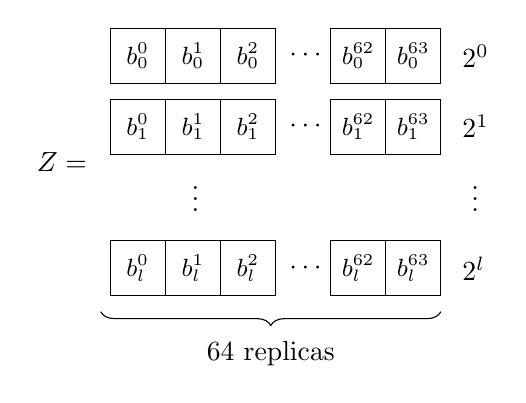
\begin{tikzpicture}

\def\boxsize{0.7}
\def\gap{0.12} % <-- horizontal spacing
\def\step{\boxsize+\gap}
\def\rowsep{0.9}

\tikzset{
    bitbox/.style={
        draw,
        minimum size=\boxsize cm,
        inner sep=0pt,
        font=\small,
        align=center
    }
}

% Left label
\node[left] at ({-0.05},{-1.5*\rowsep+0.5*\boxsize}) {$Z=$};

% Row k=0
\foreach \i/\clabel in {0/0,1/1,2/2}{
    \node[bitbox] at ({\i*\step+0.5*\boxsize},{0.5*\boxsize})
        {$b_{0}^{\clabel}$};
}

\node at ({3*\step+0.38},{0.5*\boxsize}) {$\cdots$};

\foreach \i/\clabel in {0/62,1/63}{
    \node[bitbox] at ({(4+\i)*\step+0.5*\boxsize},{0.5*\boxsize})
        {$b_{0}^{\clabel}$};
}

\node[right] at ({6*\step+0.15},{0.5*\boxsize}) {$2^0$};

% Row k=1
\foreach \i/\clabel in {0/0,1/1,2/2}{
    \node[bitbox] at ({\i*\step+0.5*\boxsize},{-\rowsep+0.5*\boxsize})
        {$b_{1}^{\clabel}$};
}

\node at ({3*\step+0.38},{-\rowsep+0.5*\boxsize}) {$\cdots$};

\foreach \i/\clabel in {0/62,1/63}{
    \node[bitbox] at ({(4+\i)*\step+0.5*\boxsize},{-\rowsep+0.5*\boxsize})
        {$b_{1}^{\clabel}$};
}

\node[right] at ({6*\step+0.15},{-\rowsep+0.5*\boxsize}) {$2^1$};

% Dots
\node at ({1.55*\step},{-1.9*\rowsep+0.5*\boxsize}) {$\vdots$};
\node at ({6.05*\step+0.4},{-1.9*\rowsep+0.5*\boxsize}) {$\vdots$};

% Row k=l
\foreach \i/\clabel in {0/0,1/1,2/2}{
    \node[bitbox] at ({\i*\step+0.5*\boxsize},{-3*\rowsep+0.5*\boxsize})
        {$b_{l}^{\clabel}$};
}

\node at ({3*\step+0.38},{-3*\rowsep+0.5*\boxsize}) {$\cdots$};

\foreach \i/\clabel in {0/62,1/63}{
    \node[bitbox] at ({(4+\i)*\step+0.5*\boxsize},{-3*\rowsep+0.5*\boxsize})
        {$b_{l}^{ \clabel}$};
}

\node[right] at ({6*\step+0.15},{-3*\rowsep+0.5*\boxsize}) {$2^{l}$};

% Bottom brace
\draw[
    decorate,
    decoration={brace,amplitude=5pt,mirror}
]
({0},{-3*\rowsep-0.2})
--
({6*\step},{-3*\rowsep-0.2})
node[midway,below=7pt] {64 replicas};
\end{tikzpicture}
\caption{An \UnsignedInt encoding 64 parallel unsigned integers. Each row is a \Bits associated with a power of 2. The value of each integer is obtained by reading the \UnsignedInt along the corresponding column. For instance, the fifth integer stored in $Z$ is $Z_4=\sum\limits_{i=0}^l b_i^4\, 2^i$.}
\label{fig:UnsignedInt}
\end{figure}
\linenumbers
In the same way as for \Bits, the \UnsignedInt data structure enables us to add, subtract or even multiply two sets of 64 integers with just the cost of one operation.\\
This implementation method has proven efficient when dealing with discrete-value models such as the Ising \cite{HFreund_1988} or the spin glass \cite{palassini1999} models, but it has not yet been employed to study the Hopfield network.

\subsection{Second Optimization: Shared random numbers}
The bitwise implementation is a structural optimization of the data representation. On top of this structural optimization can be added a physical one which consists in having all replicas share the same sequence of random numbers, fully parallelizing their evolution. This turns out to be central: random number generation is often the simulation bottleneck, as it involves costly operations such as multiplications and is called at every step of the hot loop. A schematic view of the shared random number is shown in Figure~\ref{fig:shared_rng}. Using the same random number among all evolutions raises the questions of the independence of the realizations, this will be the subject of the next subsection.
\nolinenumbers
\begin{figure}[t]
\centering

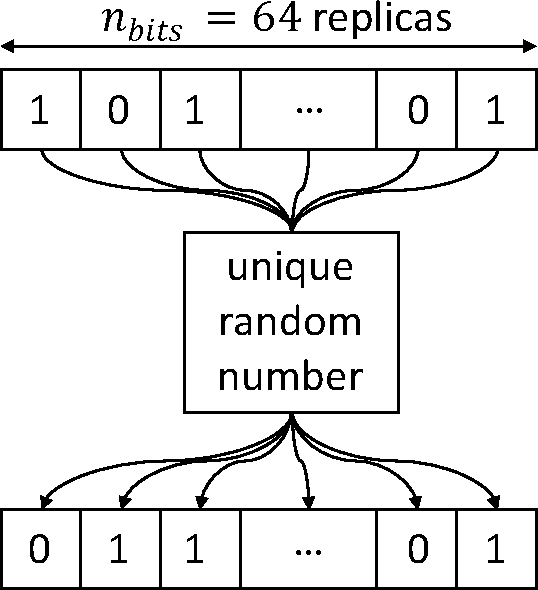
\includegraphics[width=0.5\columnwidth]{pictures/random_number.pdf}
\caption{All 64 replicas of a given spin share the same random number at each step.}
\label{fig:shared_rng}
\end{figure}
\linenumbers
\FloatBarrier
\subsection{Note on the independence of the realizations}
Because all replicas share the same sequence of random number, it is not obvious that their evolutions are independent. This is in fact guaranteed by two facts. The first one is that each replica is initialized independently of the others. The second one is that the shape of the energy landscape in each realization is also shaped independently of the others. Thus, the shared random number yields different outcome in each replica. A schematic view of this mechanism is shown in \Cref{fig:replica_independence}.
\nolinenumbers
\begin{figure}[b]
\centering

\includegraphics[width=\columnwidth]{replica_independence.png}
\caption{Schematic view of the independence of the realizations evolving from the same sequence of random numbers. Because of the unique energy landscape in every replica and the independent initializations, the same random number yields independent evolutions.}
\label{fig:replica_independence}
\end{figure}
\linenumbers
In a further analysis, one would be tempted to share the energy landscape across all replicas. This happens for instance if all replicas share the same patterns to be stored in the case of the Hopfield model, see subsection \ref{subsec:hopfield_model}. In this case, the realizations would be correlated through this shared energy landscape.
\FloatBarrier
\subsection{Standard implementation of the Metropolis algorithm}

We show here the standard implementation of the Metropolis algorithm, which will be broadly shared across all models.\\
If $\Delta E_k \leq 0$ the flip is accepted. Else, the flip condition $r \leq e^{-\beta \Delta E_k}$, yields:
\begin{equation}
\begin{aligned}
  \frac{-1}{\beta}\log r &\geq \Delta E_k\\
  \frac{-1}{\beta \kappa}\log r &\geq \Lambda_k,\\
\end{aligned}
\label{eq:flip_condition}
\end{equation}
with
\begin{equation}
  \Lambda_k \equiv \frac{\Delta E_k}{\kappa}.
  \label{eq:def_lambda}
\end{equation}
where  $\kappa$ corresponds to the constants of the model (\textit{i.e.} $2J$ in the case of the Hopfield model).
With $r \sim \mathcal{U}([0,1])$, we know that $-\log r \sim \mathcal{E}(1)$ , thus:
\begin{equation}
   \theta \equiv -\frac{1}{\beta \kappa}\log r  \sim \mathcal{E}(\beta \kappa).
\end{equation}
The left-hand side of \Cref{eq:flip_condition} is a random variable of probability density $p(\theta)=\beta  \kappa e^{-\beta  \kappa \theta}$ and mean $(\beta \kappa)^{-1}$.
The right-hand side of the equation is an integer which can be positive of negative. However, due to the first escape condition of the algorithm, we know that it is strictly positive. 
The left-hand side is thus compared with a positive integer. We can thus only consider the whole part of it without changing the inequality in order to obtain an integer-only flip condition, 
defining $q := \lfloor \theta \rfloor $:
\begin{equation}
 q\geq \Lambda_k.
  \label{eq:flip_int}
\end{equation}

A first naive implementation of the classical algorithm is given in the \Cref{alg:ising_classic_naive} in the appendix, where each of the $n_\text{bits}$ branch possesses its own random number. 
A more efficient implementation would be to share the drawn random threshold across the replicas. This shared random number version yields a fast escape condition, taking advantage of the inequality
\begin{equation*}
 -\max\Lambda_k \leq \Lambda_k \leq \max\Lambda_k ,
\end{equation*}
where $\max\Lambda_k $ only depend on the topology of the network.
Plugging this into Eq~\eqref{eq:flip_int} yields the flip escape condition:
\begin{equation}
q \geq \max\Lambda_k
 \label{eq:flip_escape_condition}
\end{equation}
When satisfied, this guarantees that Eq.~\eqref{eq:flip_int} holds for every replica regardless of its local configuration, so that all replicas are flipped simultaneously without computing the per-replica test.
This condition is typically met in the high-temperature regime, where $\theta$ is more likely to be large.\\
We show in the \Cref{alg:ising_classic} the shared random number implementation of the Metropolis algorithm. This implementation is valid for all models, provided that the definition of $\kappa$ is adapted to each model.\\
\vspace{1em}
\nolinenumbers
\begin{algorithm}[t]
\DontPrintSemicolon
\caption{Standard Metropolis implementation}
\KwIn{Lattice spins $\{S_i\}$, coupling $J$, inverse temperature $\beta$}
\KwOut{Updated lattice spins $\{S_i\}$}
\BlankLine
\BlankLine
\For{$\mathrm{sweep} = 1$ \KwTo $N_{\mathrm{sweeps}}$}{
    \For{$k = 1$ \KwTo $N$}{
      Draw $q$ with $\theta \sim \mathcal{E}(\beta \kappa)$\;
      \eIf{$q \geq \max\Lambda_k$}{
        \For{$r = 1$ \KwTo $n_\text{bits}$}{
            $s_k^{(r)} \leftarrow -s_k^{(r)}$\;
            }
        }{
            \For{$r = 1$ \KwTo $n_\text{bits}$}{
                Compute $\Lambda_k^{(r)} $\;
                \If{$\Lambda_k^{(r)} \leq 0$ \textbf{or} $q \geq \Lambda_k^{(r)}$}{
                    \BlankLine
                    \tcp{the test $\Lambda_k^{(r)} \leq 0$ is not necessary as $q$ has already been drawn, but is shown for pedagogy}
                    $s_k^{(r)} \leftarrow -s_k^{(r)}$\;
                }
            }
        }
    }
}
\label{alg:ising_classic}
\end{algorithm}
\linenumbers
\vspace{1em}
This reduces the number of random draws per $n_\text{bits}$ cycle update to just one, shared among all replicas. This optimization is possible even though the structure is not fully parallelized across replicas. The only case for which this parallelized random number optimization might not be as efficient as expected is when $\Lambda_k^{(r)} \leq 0$  for all replicas simultaneously, in which case a random threshold is drawn but never used.
The complexity of this algorithm on a given network is $\mathcal{O}\left(N_\text{sweeps}\cdot N \cdot \langle n_\text{neighbor} \rangle \cdot n_\text{bits} \right)$.
\subsection{Bitwise Implementation of the Metropolis algorithm on the Hopfield network}
Given the Hamiltonian~\eqref{eq:Hopfield}, the energy shift when flipping the neuron $S_k$ is:
\begin{equation}
  \begin{aligned}
  \Delta E_k&= 2\sum_{i\partial k}w_{ki}S_kS_i\\
            &= \frac{2}{N}  \sum_{i \in \partial k}\sum_{\mu=1}^{p}\xi_k^\mu \xi_i^\mu S_k S_i
  \end{aligned}
\end{equation}
We write $w_{ki} = \frac{1}{N}G_{ki}$ in order to deal with integer-only variables. Thus:
\begin{equation*}
    \frac{\Delta E_k N}{2} = \sum_{i \in \partial k} G_{ki} S_i S_k \qquad \text{with} \quad G_{ki} \in [-p, p].
\end{equation*}

And the flip condition becomes:
\begin{equation}
 q \geq S_k h_k,
  \label{eq:flip_condition_hopfield}
\end{equation}
with $h_k =  \sum_{i \in \partial k }G_{ki}S_i$ the local field and $q = \lfloor \theta \rfloor =-\frac{N}{2\beta} \log r$.

\subsubsection{Optimized implementation}
\label{sec:base_implementation_hopfield}
A more effective approach would be to retain the integer factor $G_{ki}$, which is suitably stored into an \UnsignedInt in the bitwise implementation. 
We operate the shift $\tilde{G}_{ki} = p + G_{ki}$, $\tilde{G}_{ki} \in [0, 2p]$ in order to deal with positive only integers, as required by the \UnsignedInt format. Then:
\begin{align*}
    \sum_{i \in \partial k} G_{ki} S_i S_k &= \sum_{i \in \partial k}(\tilde{G}_{ki}-p)(2C_{ik}-1)\\
    &= -\sum_{i \in \partial k} \tilde{G}_{ki} + 2\sum_{i \in \partial k}
     C_{ik}(\tilde{G}_{ki}-p) + n_k p,
\end{align*}
with $C_{ki}= B_k \odot B_i$.
The bitwise flip test is then:
\begin{equation}
   q+ \sum_{i \in \partial k} \tilde{G}_{ki} + 2p\sum_{i \in \partial k} C_{ki} \geq  pn_k+
    2\sum_{i \in \partial k} C_{ki}\, \oplus \tilde{G}_{ki}
\end{equation}
Where $C_{ki}\, \oplus \tilde{G}_{ik}$ consists in the XOR operator between $C_{ki}$ and every \Bits composing the \UnsignedInt $\tilde{G}_{ki}$:
\begin{equation*}
  \left(C_{ki}\, \oplus \tilde{G}_{ki}\right)_l = C_{ki} \oplus \left(\tilde{G}_{ki}\right)_l,
\end{equation*}
where $l$ denotes the $l$-th \Bits of $\tilde{G}_{ki}$ (associated with the power $2^l$).
This is strictly equivalent to setting the columns of $\tilde{G}_{ik}$ to 0 where $C_{ki}$ is zero and leave the other ones untouched. 
This method thus requires the creation of several \UnsignedInt objects, whose sizes are fixed throughout the evolution of the system. 
Also, $\tilde{G}_{ki}$ is simply determined by the pattern initialization of the system and does not depend on the spin configuration. 
It can thus be computed once before letting the system evolve, saving significant computation time. Looking at \Cref{eq:flip_condition_hopfield}, 
the escape condition that enables us to flip all replicas of the spin without considering each configuration becomes:
\begin{equation}
   q\geq p\,n_k
    \label{eq:escape_condition_hopfield_bitwise}
\end{equation}
We show in \Cref{alg:Hopfield_bitwise} the bitwise implementation of the Metropolis algorithm on the Hopfield network.
\linenumbers
\begin{algorithm}[b]
\DontPrintSemicolon
\caption{Bitwise Hopfield Metropolis}

\KwIn{Bit-replicated spins $\{B_i\}$, couplings $\texttt{Couplings}$, neighbor lists $\partial i$, number of patterns $P$}
\KwOut{Updated spin configurations $\{B_i\}$}

\BlankLine
\textbf{Preallocated variables:}
$\mathtt{Bits}\ c_{ij},\ \mathtt{mask}$\;
$\mathtt{UnsignedInt}\ \Sigma_c,\ \Sigma_{cg},\ \Sigma_g,\ \mathrm{LHS},\ \mathrm{RHS},\ tmp$\;

\BlankLine

\For{$i=1$ \KwTo $N$}{
    $\Sigma_g(i)\leftarrow 0$\;
    \For{$j\in\partial i$}{
        $\Sigma_g(i)\mathrel{+}=G_{ij}$
    }
}
\tcp*{Precompute coupling sums}

\BlankLine

\For{$\mathrm{sweep}=1$ \KwTo $N_{\mathrm{sweeps}}$}{
    \For{$\mathrm{step}=1$ \KwTo $N$}{

        Draw a random neuron $i$\;

        Draw $q$ with $\theta \sim \mathcal{E}(2\beta)$\;

        \eIf{$q \geq p\,n_k$}{
            $B_i\leftarrow\neg B_i$
            \tcp*{Unconditional flip}
        }{

            $\Sigma_c\leftarrow0$\;
            $\Sigma_{cg}\leftarrow0$\;

            \For{$j\in\partial i$}{

                $c_{ij}\leftarrow B_i\odot B_j$
                \tcp*{Replica-wise agreement}

                $\Sigma_c\mathrel{+}=c_{ij}$\;

                $tmp\leftarrow G_{ij}$\;

                $tmp\leftarrow tmp\land c_{ij}$\;

                $\Sigma_{cg}\mathrel{+}=tmp$\;
            }

            $\mathrm{RHS}\leftarrow P\,n_i+2\,\Sigma_{cg}$\;

            $\mathrm{LHS}\leftarrow \Sigma_g(i)+r+2P\,\Sigma_c$\;

            $\mathtt{mask}\leftarrow(\mathrm{RHS}\le\mathrm{LHS})$
            \tcp*{Replica-wise acceptance test}

            $B_i\leftarrow B_i\oplus\mathtt{mask}$\;
        }
    }
}
\label{alg:Hopfield_bitwise}
\end{algorithm}
\nolinenumbers
\FloatBarrier
\subsubsection{Reducing complexity in dense networks using overlaps}
In the case of a fully-connected network, summing over the neighbors of $k$ amounts to sum over the entirety of the network, yielding a complexity of $\mathcal{O}(N)$ in itself. In order to reduce this complexity, one can also make use of the overlap to compute the neuron flip condition. We define the extensive overlap:
\begin{equation}
    M^\mu= N m^\mu = \sum_{i=1}^N \xi_i^\mu S_i.
    \label{eq:extensive_overlaps}
\end{equation}
Then,
\begin{align*}
    S_kh_k &=
    \sum_{i \in \partial k} G_{ki} S_i S_k \\
    &= \sum_{\mu=1}^p \xi_k^\mu  S_k \left(M^\mu - \sum_{\substack{i \notin \partial k \\ i \neq k}}\xi_i^\mu S_i - \xi_k^\mu S_k \right)\\
    &= \sum_{\mu=1}^p \xi_k^\mu S_k M^\mu -  \sum_{\mu=1}^p \sum_{\substack{i \notin \partial k \\ i \neq k}} \xi_k^\mu \xi_i^\mu S_k S_i - \sum_{\mu=1}^p \left(\xi_k^\mu S_k \right) ^2.
\end{align*}
The second sum is simply the sum $G_{ki} S_i S_k$ over the non-neighbors of $k$. Each term of the last sum is equal to 1. The flip condition is thus:
\begin{equation}
 q+p  \geq \sum_{\mu=1}^p \xi_k^\mu S_k M^\mu - \sum_{\substack{i \notin \partial k \\ i \neq k}} G_{ki} S_i S_k.
\end{equation}
The bitwise implementation of this condition requires that all quantities are positive. We thus define the shifted extensive overlaps 
$ \tilde{M}^\mu = M^\mu + N$, $\tilde{M}^\mu \in[0, 2N]$. Then, writing $S_k \xi_k^\mu = 2 C_k^\mu -1$ with $C_k^\mu = B_k \odot X_k^\mu$, $X_k^\mu $ being the binary counterpart of $\xi_k^\mu$,
\begin{align*}
    \sum_{\mu=1}^p &\xi_k^\mu S_k M^\mu = \sum_{\mu=1}^p \xi_k^\mu S_k (\tilde{M}^\mu - N)\\
    &= - N \sum_{\mu=1}^p \left(2C_k^\mu - 1 \right) + \sum_{\mu=1}^p \left(2 C_k^\mu-1\right) \tilde{M}^\mu\\
    &= Np - 2N \sum_{\mu=1}^p C_k^\mu + 2 \sum_{\mu=1}^p C_k^\mu \oplus \tilde{M}^\mu- \sum_{\mu=1}^p \tilde{M}^\mu.
\end{align*}

We also use the previous decomposition of $G_{ki} S_i S_k$:
\begin{widetext}
\begin{equation*}
    \sum_{\substack{i \notin \partial k \\ i \neq k}} G_{ki} S_i S_k= -
    \sum_{\substack{i \notin \partial k \\ i \neq k}} \tilde{G}_{ki} +
  2 \sum_{\substack{i \notin \partial k \\ i \neq k}} C_{ik} \oplus \tilde{G}_{ki} - 2p
    \sum_{\substack{i \notin \partial k \\ i \neq k}} C_{ik}
    +(N-n_k-1)p.
\end{equation*}
The overall bitwise flip condition is thus:
\begin{equation}
   q+ 2N \sum_{\mu=1}^p C_k^\mu +  \sum_{\mu=1}^p \tilde{M}^\mu +   2 \sum_{\substack{i \notin \partial k \\ i \neq k}} C_{ik} \oplus \tilde{G}_{ki} \geq  p n_k + 2 \sum_{\mu=1}^p C_k^\mu \oplus \tilde{M}^\mu +\sum_{\substack{i \notin \partial k \\ i \neq k}} \tilde{G}_{ki} + 2p \sum_{\substack{i \notin \partial k \\ i \neq k}} C_{ik}.
    \label{eq:bitwise_flip_overlap}
\end{equation}
\end{widetext}
This flip condition only requires summing over the patterns and over the non-neighbors of the considered neuron, rather than over its full neighborhood. 
In a dense network, where $|\partial k| \gg p$, this is significantly faster than the direct computation, reducing the computational cost from $\mathcal{O}(N)$ to $\mathcal{O}(P+ |\overline{\partial k} |)=\mathcal{O}(\alpha N+ |\overline{\partial k} |)$. The downside of this method is that it requires another summation on the patterns after the flip condition computation to update the overlaps, if the neuron should be flipped: $\tilde{M}^\mu \leftarrow \tilde{M}^\mu - 2 \xi_k^\mu S_k$, with the bitwise equivalent: $\tilde{M}^\mu \leftarrow \tilde{M}^\mu + \text{mask}_k (2-4C_k^\mu)$ with $\text{mask}_k$ the \Bits object obtained from the computation of the flip condition across the $n_\text{bits}$ replicas. This implementation is thus faster than the original one when $\rho \geq \alpha + 1/2$ with $\rho$ the density of the network.
In the case of a fully-connected network, the flip condition \eqref{eq:bitwise_flip_overlap} becomes:
\begin{equation}
\begin{aligned}
   q+ 2N \sum_{\mu=1}^p C_k^\mu +  &\sum_{\mu=1}^p \tilde{M}^\mu \geq \\ & p (N-1) + 2 \sum_{\mu=1}^p C_k^\mu \oplus \tilde{M}^\mu,
    \label{eq:bitwise_flip_overlap_FC}
\end{aligned}
\end{equation}
and no summation over the non-neighbors is required. We present this implementation in \Cref{alg:Hopfield_bitwise_overlaps}.


